\chapter{Mathematical Background}
\label{appendix: B}

\emph{Appendix B displays the mathematical background of the used Python packages and statistics.}

\section{Python Packages}

\subsection{Pastas}
Pastas is a Python package made to analyze a sequence of data points that are collected over specific intervals of time \cite{collenteur-2019}. Data gaps are present in the dataset, resulting in potential problems later on in the development of the model. A first step is to execute a system analysis, where possible hydrological variables are determined. Continuing with the model construction, it is determined how variables are transferred to fluctuations. In the end, the model has to be approved to see which variables have actual influence on model performance.

The time series model can be described in the most general way:\\
\\
\begin{figure}[htbp]
    \centering
    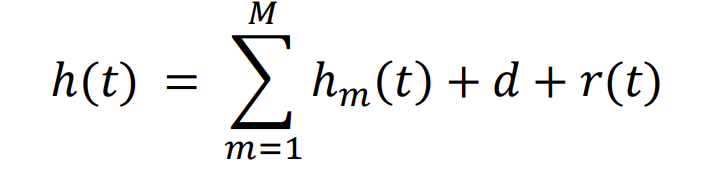
\includegraphics[width=0.5\linewidth]{appendix/basic model.png}
    \caption{Formula for a basic time series model \cite{asmuth-2021}.}
    \label{Pastas}
\end{figure}\\
\\
\(H\) displays the groundwater level, \(hm(t)\) is the contribution of influence \(m\), \(d\) is the base level of the model, and \(r\) are the model residues. The total influence that contributes to the groundwater level fluctuations is \(M\) \cite{asmuth-2021}. 


\subsection{PySensors}
PySensors is a Python package for scalable optimization of monitoring well placement from observed data. The package provides a tool for sparse sensor placement optimization approach that ensures a data-driven dimensionality reduction \cite{manohar-2018}. The developed method ensures near optimal placement for decision-making tasks, like the placement of monitoring wells. An advantage is that the method can be adapted to be suitable for different optimization algorithms and objective functions. Generally, the PySensors package is applied for reconstruction measures, to recover a high dimensional signal from a limited number of measurements. The foundation of the package computes data by using powerful dimensionality reduction techniques as the principal component analysis (PCA) and random projections. PySensors can be used for classification purposes by implementing the Sparse Sensor Placement Optimization for Classification algorithm (SSPOC). This algorithm provides a compressed sensing optimization that makes it possible to allow one to optimize sensor placement for classification accuracy, but can also identify the sparsest set of sensors that reconstructs a ‘discriminating plane’ in a feature subspace. The implementation of the SSPOC algorithm is a general algorithm that can be used simultaneously with a linear classifier (an algorithm that separates two types of objects by a line or hyperplane) \cite{manohar-2018}. The PySensors package can also implement the Sparse Sensor Placement Optimization for Reconstruction method for recovering high-dimensional signals \((x)\) from linear sensor measurements in the form: \\
\\
\(y = Cx\)\\
\\
The optimal measurements of \(x\) are identified and given by operator \(C\), which describes the components of \(x\) to observe. The SSPOR method has its purpose to find the best subset of available measurements from which the full signal can be received in the estimation problem. 
\begin{figure}[htbp]
    \centering
    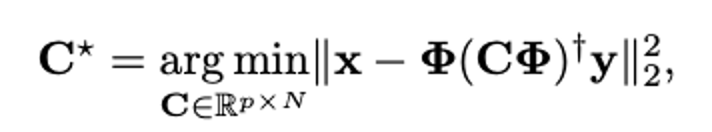
\includegraphics[width=0.5\linewidth]{appendix/pysensors.png}
    \caption{Formula of the Sparse Sensor Placement Optimization for Reconstruction algorithm \cite{manohar-2018}.}
    \label{Pysensors}
\end{figure}
According to De Silva, PySensors provides methods to enable straightforward exploration of the impacts of critical hyper parameters, such as the number of sensors or basic modes \cite{silva-2021}. In this case, those are the number of monitoring wells. 

\section{Statistics}
\subsection{Welch's t-Test}
In a Welch’s t-Test, two data groups can be compared within the dataset without assuming equal data variances of both data groups. A t-Test is carried out to criticize whether a dataset with a combination of measurement types as data logger and manual collection methods are recommended to be used in the model. A Welch’s t-Test is a suitable approach, because the denominator of the formula provides the possibility that the two data groups have unequal variances. The t-Test is determined by the mean of the two data groups, the variances of both data groups, and the sample size of the two data groups. Since a difference is detected between the data quantity of the data loggers and the manual collection method, a Welch’s t-Test is a suitable measure to determine if there is actually a significant difference between the two data groups. The t-Test is based on the following formula \cite{jung-2020}, see figure \labelcref{T-test}.
\begin{figure}[htbp]
    \centering
    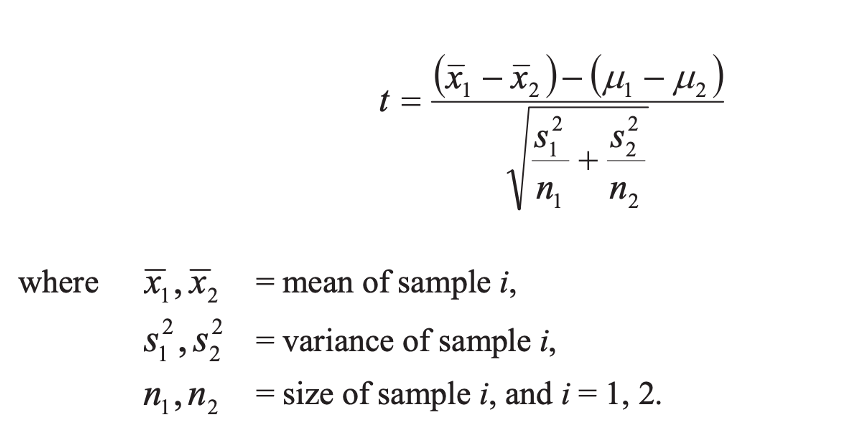
\includegraphics[width=0.5\linewidth]{appendix/welch.png}
    \caption{Formula to calculate t in the Welch's t-test \cite{jung-2020}.}
    \label{T-test}
\end{figure}
\noindent
Where t is a combination of the properties that are combined into the t-statistic, a random variable. \(X1\) and \(X2\), which can be explained as the mean of the sample \(i\), in this case the mean of the groundwater level of the data loggers and the manual collection method. \(U1\) and \(U2\) can be explained as the population means, the theoretical means, which are assumed from the samples that are taken. The denominator can be described as the root of variance of the data loggers divided by the sample size of the data loggers plus the variance of the mean collection method divided by the sample size of the mean collection method \cite{jung-2020}. 
\noindent
In this context an \(alpha = 0.05\) is chosen, where a \(P-value < 0.05\) indicates evidence against the null hypothesis and suggests if there is a statistically significant relationship. The alpha threshold is arbitrary, meaning that a higher or lower alpha than 0.05 possibly depends on the context. An alpha of 0.05 manages the risk of rejecting the null hypothesis, while maintaining sufficient power to detect accurate results. The result of the t-Test, the p-value, generally does not provide much information about the magnitude or importance of the observed effect. If a p-value is lower than 0.05, the result suggests that the observed data does not provide sufficient evidence against the null hypothesis and indicates a statistically significant effect between the researched variables \cite{statistics-easily-2024}. 
 

\subsection{QR factorization}
QR Factorization is a mathematical approach that breaks down matrix \(A\) into the product of two matrices: \(Q\) and \(R\).  Matrix \(A\) is an \(m*n\) matrix with linearly independent columns. The Gram-Schmidt orthogonalization process results in producing \(Q\), with orthonormal columns, and \(R\), an upper triangular matrix with positive entries on the diagonal. \(Q\) transforms the original dataset into a new dataset with independent columns. This action is essential for evaluating the unique contribution of each monitoring well. The triangular matrix of \(R\) serves to rank monitoring wells based on their informational relevance \cite{university-of-regina-no-dateA}. Figure \labelcref{QR} displays the decomposition of matrix A into matrix Q and R \cite{harp-no-date}.
\begin{figure}[htbp]
    \centering
    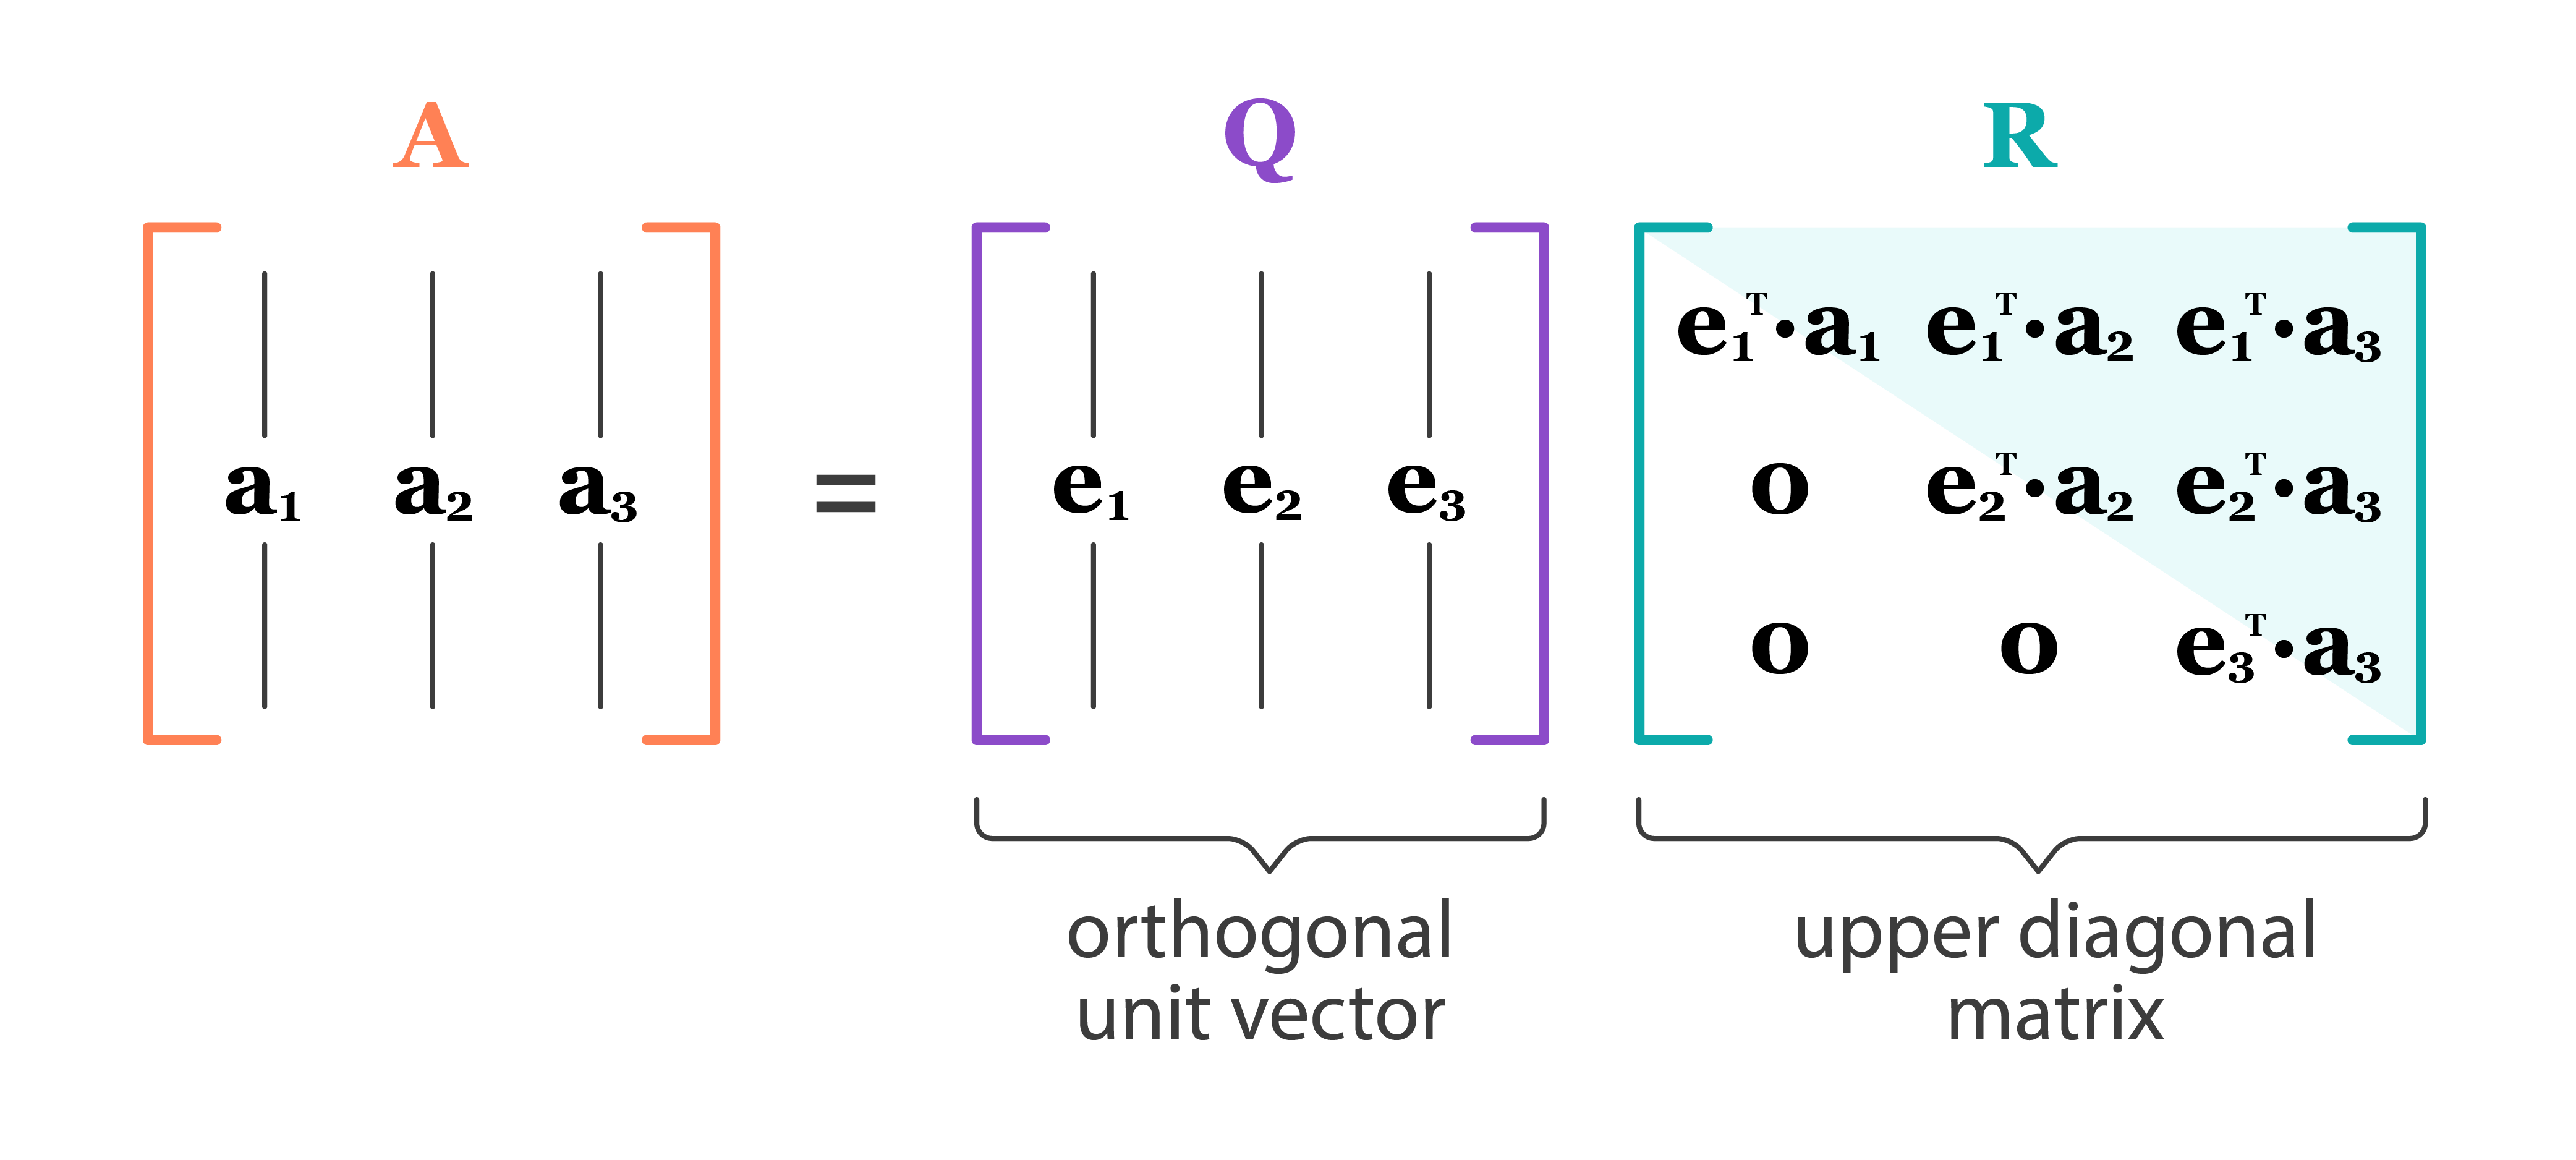
\includegraphics[width=0.5\linewidth]{appendix/qrfac.png}
    \caption{QR factorization or decomposition of the matrix A into an orthogonal matrix Q and triangular matrix R \cite{harp-no-date}.}
    \label{QR}
    
\end{figure}

%Q is an orthogonal matrix that transforms the original dataset into a new dataset with independent columns. This is essential for evaluating the unique contribution of each monitoring well. On the other hand, R is a triangular matrix, where values below the diagonal are equal to zero. The triangular matrix serves to rank monitoring wells based on their informational relevance. Figure 4.1, visualizes the decomposition of product A into matrices Q and R. 

\subsection{Genetic Algorithm}
A genetic algorithm (GA) is based on decision variables that are encoded as binary strings, genes, for a given location - in this case the municipal area of Rotterdam. Combinations of the genes generate chromosomes which correspond to possible monitoring networks. Random chromosomes evolve to network generations. In each generation, the fitness of the “population” is evaluated. Chromosomes are selected based on their fitness on the current population and modified using genetic operators. The approach is based on ‘survival-of-the-fittest’ \cite{hermawanto-2013}. The network of monitoring wells corresponds to ‘chromosomes’ and each monitoring well in the network is represented by a binary bit that determines if the well will be selected for the network or not (1 = yes, 0 = no). Every unique monitoring well is evaluated by the fitness of the network by an inverse distance and interpolation approach. GA are stochastic optimization tools that work on Darwinian models and are capable of solving near-optimal solutions for multi variable functions without the usual mathematical requirements \cite{ayvaz-2018}.

\begin{figure}[htbp]
    \centering
    
\includegraphics[width=0.70\linewidth]{appendix/ga.png}
    \caption{Formula to determine the genetic algorithm in the optimization model \cite{koshikawa-2020}.}
    \label{GA}

\end{figure}








